
\section{Problem 2: Momentum Modeling and Evaluation of Long Short-Term Memory Networks (MM-LSTM)}

\subsection{Stochastic Probability Based Winner Prediction}

In order to assess whether momentum plays any role in the match, we first develop a stochastic probability-based prediction model of winning percentage. We choose three empirical metrics to parameterize this stochastic probability model:
\begin{itemize}[label=\textbf{\normalsize$\bullet$}]
    \item $P_{base}$: the win rate value of a player base, set to a fixed value of 0.5.
    \item $P_{server}$: the portion of a player's win rate that is increased over the base win rate as a server.
    \item $m_i$: the strength value of $player_i$.
    \item $P_{factors}$:the probability change value caused by factors.
\end{itemize}

The computation of $P_{server}$ and $m_i$ is described below in turn:

For $P_{server}$, we analyzed the win rates of players as servers based on the data set of Wimbledon 2023 Gentlemen's singles matches after the second round provided by MCM. It was found that the probability of winning as a server decreases over the different sets of a match, suggesting that the effect of the serve on a player's win decreases as the match progresses. Also based on the analysis of the paper by researchers at the University of Amsterdam \cite{p_server}, we integrate both and decide to only consider the impact of the serving position in the first two games.

We have done a statistical analysis of the probability of a server winning in the data set, and the base value of the increase in the probability of a player winning by serving is 0.173119165. Based on this, we modeled the $P_{server}$ formulation as follows:

% % 描述先决条件中基础概率与发球手位置增加的概率
% \begin{equation}
% R_{server}=0.173119165
% \end{equation}
% % 在这里指出发球位置对于胜利的影响
% \[ P_{server} = \left\{
% \begin{array}{ll}
% 2 \cdot R_{server}, & \text{set\_no} = 1 \\
% R_{server}, & \text{set\_no} = 2 \\
% 0, & \text{set\_no} > 2
% \end{array}
% \right.
% \]

\begin{equation}
R_{server}=0.173119165
\end{equation}
\begin{equation}\left.P_{server}=\left\{\begin{array}{ll}2\cdot R_{server},&\text{set\_no}=1\\R_{server},&\text{set\_no}=2\\0,&\text{set\_no}>2\end{array}\right.\right.\end{equation}

Similarly, for other factors, we also use similar methods for analysis, and ultimately use the following formula to calculate:
\begin{equation}
 \sum P_{factors} = P_{server} + \sum P_{others} 
\end{equation}

For $m_i$, we take the ratio of the final scores and other factors of two players in a game as the relative ratio of their strengths, based on which we calculate the strength intensity of each player as the value of $m_i$. The specific steps are as follows:


\begin{enumerate}
  \item Initialize the player list, set two attributes for each player: relative\_strength, strength\_ratio. relative\_strength is a list of the relative strength of the players, set its initial value to 100; strength\_ratio Indicates the relative ratio of strength between the player as player1 and the corresponding player2.
  \item Iterate through Wimbledon\_featured\_matches.csv, get the player1, player2, p1\_point\_won and p2\_point\_won at the end of each match. For each player1, the value of p1\_point\_won divided by p2\_point\_won is recorded in strength\_ratio as its strength relative to player2.
  \item Iterate through the list of players and get the relative\_strength of the current player, recorded as player1\_strength. Calculate the player2\_strength of the corresponding player2, whose value is equal to player1\_strength * ratio. After that, add the calculated play2\_strength to the relative\_strength list of player2.
  \item Iterate through the list of players, and if the player's relative\_strength has more than one value, take the average of the values and use it as the new relative\_strength.
  \item Scales the relative\_strength of each player to a value between 0 and 100.
\end{enumerate}

% The pseudo-code description of the above process is shown in Algorithm \ref{algo:player_strength}:


% \begin{algorithm}
% \footnotesize
% 	\caption{Calculation of Player Strength Value $S_i$}
% 	\label{algo:player_strength}
% 	\begin{algorithmic}[1]
% 		\Require Competition data $D_f$
% 		\Ensure Relative strength of players in k matches $S = \{S_1, S_2, \dots , S_k\}$
%         \Function{$GetStrengthRatios$}{$D_f$}:
% 			\For{each $Match_i$ of $D_f.Matchs$}
%                     \If{$Match_i \in D_f.Player.Type$}
%                         \State $Ratios \gets $ $\frac{Match_i.Point[0]}{Match_i.Point[1]}$
%                     \EndIf
%                 \EndFor
% 		      \State \Return $Ratios$
% 		\EndFunction\\
    
%         \Function{$GenerateStrengthRatios$}{$Ratio_i, Players$}:
% 			\State $Strength \gets Initialization()$
%                 \For{$Player \text{ of } Players$}
%                     \If{$Ratios\_i.label \in Player.name$}
%                 \State $Strength \gets Ratios\_i.data \times Player.Ratio$
%             \EndIf
%         \EndFor
%         \State \Return $Strength$
% 		\EndFunction\\
  
% 		\State $StrengthRatios \gets  GetStrengthRatios(D_f)$
%         \For{each $D_{f_i}$ of $D_f$}
%             \State $Players \gets  D_{f_i}.Player1 , D_{f_i}.Player2$
%             \For{each $Ratio_i$ of $StrengthRatios$}
%                 \If{$Ratio_i \in D_f.Ratios$}
%                     \State $S_i \gets GenerateStrengthRatios(Ratio_i, Players)$
%                 \EndIf
%             \EndFor
%         \EndFor\\

%         \State $S \gets ScoreStandardize(S)$\\
%         \Return S
% 	\end{algorithmic}
% \end{algorithm}


Based on the obtained $P_{server}$ and $m_i$ above, we model the probability of player1 winning under stochastic probability as follows:

% 在随机概率下,play1获胜的概率
\begin{equation}P_{1} = \frac{\left( P_{base} + \sum P_{factors} \right)\cdot m_{1}}{\left( P_{base} +\sum P_{factors}  \right) \cdot  m_{1} +\left( P_{base} -\sum P_{factors} \right) \cdot m_{2} } 
\end{equation}


% The traditional momentum model is formulated as follows:
% \begin{equation}
% \begin{aligned}
% p_* & =\sum p_i \\
% & =\sum m_i v_i
% \end{aligned}
% \end{equation}

\subsection{An LSTM Model is Equivalent to a Momentum-Based Model}\label{sec:momentum_lstm}
To illustrate the correlation between our LSTM model and momentum, we simplify the modeled LSTM model into a well-formed momentum model based on the following equations.

Our LSTM model is formulated as follows, where $I_t$, $F_t$, $O_t$, $C_t$ represent the input gate, forget gate, output gate, Cell state mentioned in Section \ref{sec:model_structure}, respectively:
\begin{equation}
\begin{gathered}
    H_{t} = O_{t} \cdot \tanh(C_{t}) = O_{t} \cdot \tanh\left(F_{t} \cdot C_{t-1} + I_{t} \cdot \tilde C_{t}\right) \label{eq:lstm_base}
\end{gathered}
\end{equation}

Based on the formula for input gate, forget gate, output gate mentioned in \ref{sec:model_structure}, we can expand the formula \ref{eq:lstm_base}:
\begin{equation}
\begin{gathered}
    H_{t} = \sigma(x_{t} \cdot k_{5} + h_{t-1} \cdot k_{6} + b_{3}) \cdot \tanh\left(\sigma(x_{t} \cdot k_{3} + h_{t-1} \cdot k_{4} + b_{2}) \cdot C_{t-1} \right.\\
    \quad \left. + \sigma(x_{t} \cdot k_{1} + h_{t-1} \cdot k_{2} + b_{1}) \cdot \tanh\left(x_{t} \cdot k_{7} + h_{t-1} \cdot k_{8} + b_{4}\right)\right)\label{eq:lstm_expand}
\end{gathered}
\end{equation}

Simplify the formula \ref{eq:lstm_expand}:
\begin{equation}
f_{i}(x_{t}) = x_{t}\cdot k_{a_{i}(t)} + h_{t-1} \cdot k_{b_{i}(t)} + b_{c_{i}(t)}
\end{equation}
% 这是使用f代替后的表达式
\begin{equation}H_{t} = \sigma\left( f_{1}(x_{t}) \right) \cdot \tanh\left( \sigma(f_{2}(x_{t})) \cdot C_{t-1} + \sigma(f_{3}(x_{t})) \cdot \tanh(f_{4}(x_{t})) \right)\label{eq:lstm_simply}
\end{equation}

We extract a part of the formula \ref{eq:lstm_simply}, denoted $P_n$:

% 三个公式全都对齐
% \begin{equation}\begin{aligned}P_n&=\sigma(f_2(x_t))\cdot C_{t-1}+\sigma(f_3(x_t))\cdot\tanh(f_4(x_t)))\\&=F_2(x_t)C_{t-1}+F_3(X_t)\cdot\tanh(f_4(X_t))\\&=A+B\cdot\tan h(F_4(x_t))\\&=A+\alpha(p)\\
% A&=F_2(x_t)C_{t-1}+F_3(X_t)\\B&=F_3(x_t)\end{aligned}\end{equation}

% 三个公式不对齐
% \begin{equation}\begin{aligned}P_n&=\sigma(f_2(x_t))\cdot C_{t-1}+\sigma(f_3(x_t))\cdot\tanh(f_4(x_t)))\\&=F_2(x_t)C_{t-1}+F_3(X_t)\cdot\tanh(f_4(X_t))\\&=A+B\cdot\tan h(F_4(x_t))\\&=A+\alpha(p)\end{aligned}\end{equation}
\begin{equation}\begin{aligned}P_n&=\sigma(f_2(x_t))\cdot C_{t-1}+\sigma(f_3(x_t))\cdot\tanh(f_4(x_t)))\\&=F_2(x_t)C_{t-1}+F_3(X_t)\cdot\tanh(f_4(X_t))\end{aligned}\end{equation}


Then we simply $P_n$:
% \begin{equation}A=F_2(x_t)C_{t-1}+F_3(X_t)\end{equation}
% \begin{equation}B=F_3(x_t)\end{equation}
% \begin{equation}P_n=A+B\cdot\tanh(F_4(x_t))=A+\alpha(p)\end{equation}
% \begin{equation}\begin{aligned}P_n&=A+B\cdot\tanh(F_4(x_t))\\&=A+\alpha(p)\end{aligned}\end{equation}
% \begin{equation}\begin{aligned}P_n&=\sigma(f_2(x_t))\cdot C_{t-1}+\sigma(f_3(x_t))\cdot\tanh(f_4(x_t)))\\&=F_2(x_t)C_{t-1}+F_3(X_t)\cdot\tanh(f_4(X_t))\\&=A+B\cdot\tanh(F_4(x_t))\\&=A+\alpha(p)\end{aligned}\end{equation}

\begin{equation}
\left\{
\begin{aligned}
    A &= F_2(x_t)C_{t-1}+F_3(X_t) \\
    B &= F_3(x_t) \\
    P_n &= A+B\cdot\tanh(f_4(x_t)) \\
    &= A+\alpha(p)
\end{aligned}
\right.
\end{equation}

Thus, we can divide the formula in \ref{eq:lstm_simply} into two parts, $F_1$, $P_n$. $F_1$ denotes the function of the race at the current point in time, and $P_n$ denotes the temporal part, which includes the content of the cell state in the LSTM, i.e., the effect of the previous race situation on the athlete.
\begin{equation}F_{i}(x_t)=\sigma(f_i(x_{t}))\end{equation}
\begin{equation}H_{t}=F_1(x_{t})\cdot\tanh(P_{n})\end{equation}
\begin{equation}
\label{ll}
P_n=A+\alpha(p)\\\end{equation}
% \begin{equation}
% \left\{
% \begin{aligned}
%     F_{1}(x_t) &= \sigma(f_1(x_{t})) \\
%     P_n &= A+\alpha(p) \\
%     H_{t} &= F_1(x_{t})\cdot\tanh(P_{n})
% \end{aligned}
% \right.
% \end{equation}
The $\alpha(p)$ in the timing part $P_n$ represents the effect of momentum on the player during the match. This momentum consists of two components: one is the hard power of the player, and the other is the soft power of the player (e.g., scoring, the effect of the opponent on the player's mood during the match, etc.).

At this point, we have modeled the LSTM model in Section \ref{sec:model_structure} into a momentum-based model, which we call MM-LSTM.


\subsection{Comparison of Stochastic Probability Model and Momentum-Based Model}

In order to compare the random probability model and the momentum-based model, we calculated the accuracy of these two models for point win/loss prediction on a test match separately. The mean accuracy of all match predictions is presented in Table \ref{tab:mean_acc}, and the results for individual match accuracies are illustrated in Figure \ref{fig:acc_lstm_stochastic}.

\begin{table}[h]
% \begin{table*}
	\centering
	\caption{Mean Prediction Accuracy of Models} 
        \vspace{8pt}
	\label{tab:mean_acc}
	\begin{tabular}{c|c}
		\toprule[1.5pt]
  % \specialrule{.1em}{0em}{0em} % 添加粗分割线
		Model & Mean Accuracy\\
        % \specialrule{.1em}{0em}{0em} % 添加粗分割线
		\midrule[1pt]
		Stochastic Probability Model & 67.776\% \\
		Momentum-Based LSTM Model & 94.229\% \\
% \specialrule{.1em}{0em}{0em} % 添加粗分割线
		\bottomrule[1.5pt]
	\end{tabular}
\end{table}
% \end{table*}

\begin{figure}[h]
    \centering
    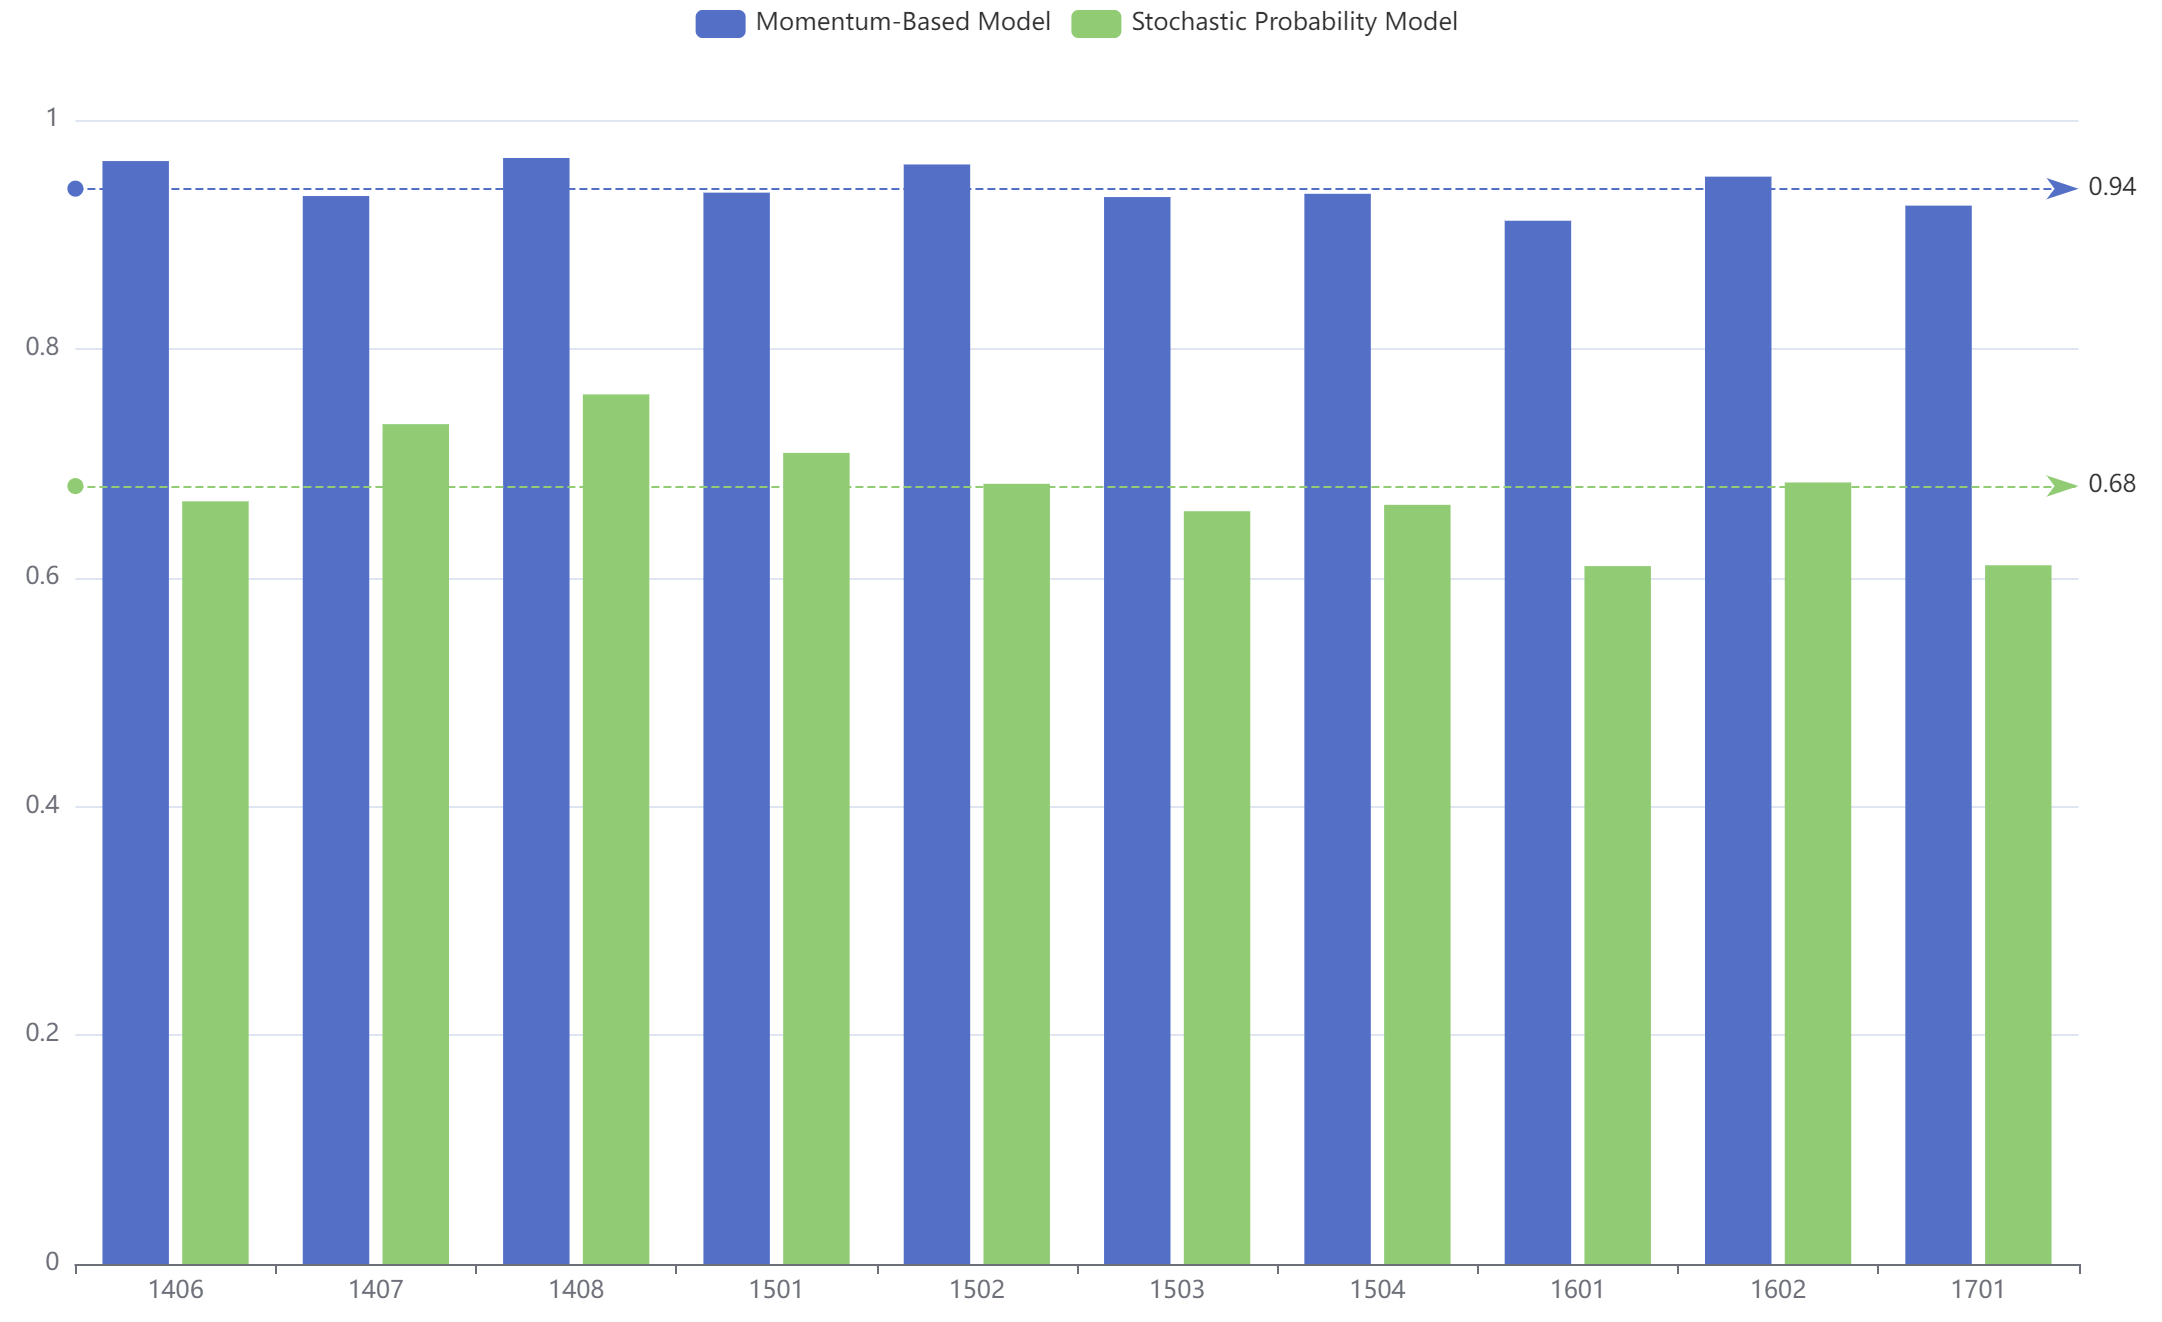
\includegraphics[width=0.8\textwidth]{figure/acc_lstm_stochastic.png}
    % \vspace{-0.3cm}
    \caption{Prediction Accuracy of Stochastic Probability Model and Momentum-Based Model 
    \textnormal{}}
    \label{fig:acc_lstm_stochastic}
    % \vspace{-0.5cm}
\end{figure}

As shown in Table \ref{tab:mean_acc}, our momentum-based model outperforms the random probability model with about 25\% accuracy. Based on this, we conclude that momentum plays a role in the game process and can be used to predict the winners and losers of the players.